\section{函数域}\label{sec:function-fields}

上一节说过, 仿射簇的维数应当衡量其坐标环中代数独立元素的最大个数. 然而, 在 $K$-代数中处理代数相关与代数独立往往相当困难, 而在 $K$ 的域扩张中处理这些概念则容易许多. 因此, 本节研究怎样从不可约仿射簇 $X$ 过渡到一个相应的域 $K(X)$, 即它的函数域.

\begin{Definition}{函数域}\leavevmode\label{def:function-field}
设 $X$ 是不可约仿射簇. $X$ 的\emph{函数域}记为 $K(X)$, 它是 $X$ 的坐标环的分式域:
\[
  K(X)=\operatorname{Frac}(K[X]).
\]
$K(X)$ 的元素称为 $X$ 上的\emph{有理函数}.
\end{Definition}

回忆一下, 分式域在第~\ref{sec:unique-factorization-polynomial-rings}~节定义. 我们在那里知道, $K(X)$ 的元素是 $f/g$ 形式的商, 其中 $f,g\in K[X]$ 且 $g\neq0$. 两个分式 $f_{1}/g_{1}$ 和 $f_{2}/g_{2}$ 相等, 当且仅当 $f_{1}g_{2}=f_{2}g_{1}\in K[X]$. 分式域的确是一个域, 其加法与乘法定义为
\[
  \frac{f_{1}}{g_{1}}+\frac{f_{2}}{g_{2}}
    =\frac{f_{1}g_{2}+f_{2}g_{1}}{g_{1}g_{2}}
  \qquad\text{和}\qquad
  \frac{f_{1}}{g_{1}}\cdot\frac{f_{2}}{g_{2}}=\frac{f_{1}f_{2}}{g_{1}g_{2}}.
\]
由于只有整环才有分式域 (Exercise~\ref{ex:fraction-field-needs-domain}), 函数域只对不可约仿射簇定义. 来看几个例子.

\begin{Example}{仿射空间的函数域}\leavevmode\label{ex:function-field-of-affine-space}
由于 $\mathbb{A}^{n}$ 的坐标环是 $K[x_{1},\ldots,x_{n}]$, 它的函数域就是通常的有理函数域
\[
  K(\mathbb{A}^{n})=K(x_{1},\ldots,x_{n}),
\]
我们已经在第~\ref{sec:unique-factorization-polynomial-rings}~节遇到过它.
\end{Example}

\begin{Example}{$\mathcal{V}(x^{2}-y^{3})$ 的函数域}\leavevmode\label{ex:function-field-of-cusp}
令 $X=\mathcal{V}(x^{2}-y^{3})\subseteq\mathbb{A}^{2}$. 计算坐标环, 得到
\[
  K[X]=K[x,y]/\langle x^{2}-y^{3}\rangle
  \quad\Longrightarrow\quad
  K(X)=\operatorname{Frac}(K[x,y]/\langle x^{2}-y^{3}\rangle).
\]
这看上去是个相当复杂的域, 但我们可以把它与一个更熟悉的域认同. 考虑 $K$-代数同态
\[
  \begin{aligned}
    \phi:K[X]&\to K[t],\\
    [f(x,y)]&\mapsto f(t^{3},t^{2}).
  \end{aligned}
\]
这是 Example~\ref{ex:cusp-bijective-map-not-isomorphism} 所定义的多项式映射的拉回. 注意 $\phi$ 是单射, 但不是同构, 因为多项式 $t$ 不在它的像里.

过渡到函数域, 就能把 $\phi$ 扩张成域同态
\[
  \begin{aligned}
    \overline{\phi}:K(X)&\to K(t),\\
    \frac{[f(x,y)]}{[g(x,y)]}&\mapsto\frac{f(t^{3},t^{2})}{g(t^{3},t^{2})}.
  \end{aligned}
\]
现在可以做除法了, 就会发现 $t$ 实际上在 $\overline{\phi}$ 的像中:
\[
  t=\frac{\phi([x])}{\phi([y])}
    =\overline{\phi}\left(\frac{[x]}{[y]}\right).
\]
这样便能求出 $\overline{\phi}$ 的逆:
\[
  \overline{\phi}^{-1}\left(\frac{f(t)}{g(t)}\right)
    =\frac{f([x]/[y])}{g([x]/[y])}
    =\frac{[y^{\max(\deg(f),\deg(g))}f(x/y)]}
          {[y^{\max(\deg(f),\deg(g))}g(x/y)]},
\]
其中第二个等号只是清除 $f$ 和 $g$ 中的分母, 使像显式地表示成 $K(X)$ 的一个元素. 由此得到 $K(X)\cong K(t)$. 建议读者在 Exercise~\ref{ex:verify-cusp-function-field-isomorphism} 中检查论证的细节.

这个例子表明, 尽管 $X$ 与 $\mathbb{A}^{1}$ 不同构, 它们的函数域却同构, 因为两者都同构于 $K(t)$. 因此, 尽管坐标环包含了关于仿射簇同构类的全部信息, 过渡到函数域时却会丢掉一部分信息.
\end{Example}

\begin{BookFlowNote}[l]{%
在前两个例子中, 所考察的两个函数域都同构于通常的有理函数域 $K(x_{1},\ldots,x_{d})$, 其中 $d$ 为某个整数. 若一个不可约簇的函数域同构于通常的有理函数域, 就称这个簇为\emph{有理}的.
}
\noindent 尽管具有同构函数域的仿射簇未必同构, 第~\ref{chap:rational-maps}~章将说明它们\textquotedbl{}双有理\textquotedbl{}.

事实上有理簇相当特殊. 本书范围之外的一个一般事实是, \textquotedbl{}大多数\textquotedbl{}簇都不是有理的. 特别是, 若 $f\in K[x_{1},\ldots,x_{n}]$ 是一个次数足够高的\textquotedbl{}随机\textquotedbl{}多项式, 则 $\mathcal{V}(f)$ 不是有理的. 下一个例子或许是最简单的非有理簇例子.
\end{BookFlowNote}

\begin{Example}{$\mathcal{V}(x^{3}+y^{3}+1)$ 不是有理的}\leavevmode\label{ex:fermat-cubic-not-rational}
\BookPairedFigure
  {置 $K=\mathbb{C}$, 令 $X=\mathcal{V}(x^{3}+y^{3}+1)\subseteq\mathbb{A}^{2}$. $X$ 的实点在\hyperref[fig:nonrational-cubic-real-points]{右图}中画出. 我们证明 $X$ 不是有理的. 论证的关键在于以下事实: 若非零多项式 $f_{1},f_{2},f_{3}\in K[x_{1},\ldots,x_{n}]$ 满足 (i) 任意两个都没有公共不可约因子, 且 (ii) $f_{1}^{3}+f_{2}^{3}+f_{3}^{3}=0$, 则 $f_{1},f_{2},f_{3}$ 必须都是常数 (证明见 Exercise~\ref{ex:polynomial-fermat-cubes}).}
  {\phantomsection\label{fig:nonrational-cubic-real-points}%
   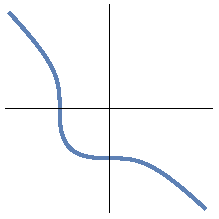
\includegraphics[width=\linewidth]{figures/function-field-nonrational-curve.pdf}}
要证明 $X$ 不是有理的, 首先注意到 $x^{3}+y^{3}+1$ 不可约, 因此
\[
  \begin{gathered}
    K[X]=K[x,y]/\langle x^{3}+y^{3}+1\rangle\\
    \Longrightarrow\quad K(X)=\operatorname{Frac}(K[x,y]/\langle x^{3}+y^{3}+1\rangle).
  \end{gathered}
\]
设
\[
  \phi:K(X)\to K(x_{1},\ldots,x_{d})
\]
对某个 $d>0$ 是域同态. 我们证明 $\operatorname{im}(\phi)\subseteq K$, 从而 $\phi$ 不可能是同构. 注意 $\phi([x])=f/g$ 且 $\phi([y])=h/k$, 其中 $f,g,h,k\in K[x_{1},\ldots,x_{d}]$ 是多项式, $g,k\neq0$. 由于 $K[x_{1},\ldots,x_{n}]$ 是 UFD, 我们可以将每个多项式分解成不可约因子的乘积并约分. 换句话说, 可以假设 $f$ 和 $g$ 之间, 以及 $h$ 和 $k$ 之间, 都没有公共不可约因子. 由 $[x^{3}+y^{3}+1]=0\in K(X)$ 得到关系
\[
  0=\phi([x^{3}+y^{3}+1])
    =\left(\frac{f}{g}\right)^{3}+\left(\frac{h}{k}\right)^{3}+1.
\]
消去分母得
\begin{equation}\label{eq:nonrational-cubic-cleared-denominators}
  (fk)^{3}+(gh)^{3}+(gk)^{3}=0.
\end{equation}
等式 \eqref{eq:nonrational-cubic-cleared-denominators} 给出 $g^{3}\mid(fk)^{3}$. 由于假设 $f$ 和 $g$ 没有公共不可约因子, 所以 $g^{3}\mid k^{3}$. 类似地, 可得 $k^{3}\mid g^{3}$. 因此, 由 $g^{3}\mid k^{3}$ 和 $k^{3}\mid g^{3}$ 知道 $g^{3}=ak^{3}$, 其中 $a$ 为常数. 将其代入等式 \eqref{eq:nonrational-cubic-cleared-denominators} 并约去 $k^{3}$, 得到关系
\begin{equation}\label{eq:nonrational-cubic-coprime-relation}
  f^{3}+ah^{3}+g^{3}=0.
\end{equation}
注意 $g$ 的不可约因子和 $k$ 的不可约因子相同, 因而按假设, 它们既不是 $f$ 的不可约因子, 也不是 $h$ 的不可约因子. 此外, $f$ 和 $h$ 不能有公共不可约因子, 否则由等式 \eqref{eq:nonrational-cubic-coprime-relation}, 它也会是 $g$ 的不可约因子, 与关于 $f$ 和 $g$ 的假设矛盾. 因此, 等式 \eqref{eq:nonrational-cubic-coprime-relation} 中任意两项都没有公共不可约因子, 可以应用 Exercise~\ref{ex:polynomial-fermat-cubes} 得到 $f,g,h,k$ 都是常数, 正如所断言的那样.

上面的论证表明, 对任意 $d>0$, $K(X)$ 都与 $K(x_{1},\ldots,x_{d})$ 不同构. 但若 $d=0$ 呢? 由于 $X$ 有不止一个点, 可知 $K\subsetneq K[X]$, 这蕴含 $K\subsetneq K(X)$, 从而 $K(X)$ 与 $K$ 不同构. 结合前面的论证, 可知 $X$ 不是有理的.
\end{Example}

最后对术语作一个简短说明: 虽然 $K(X)$ 的元素称为有理函数, 但它们实际上不是 $X$ 上的函数. 具体地说, 给定 $f/g\in K(X)$ 且 $g\neq0$, 对某些 (但非全部) $a\in X$, 可能有 $g(a)=0$. 因而 $f/g$ 只在 $X$ 中满足 $g\neq0$ 的子集上定义了一个函数. 通常用虚线箭头表示有理函数, 提醒读者它们并非在整个定义域上都有定义:
\[
  \frac{f}{g}:X\mathrel{\rightdasharrow}K.
\]
若把定义域限制为 $\mathcal{V}(g)$ 的补集, 则每个有理函数都会给出一个真正的函数, 为定义域的每个元素指定一个值:
\[
  \frac{f}{g}:X\setminus\mathcal{V}(g)\longrightarrow K.
\]
这个概念和记号将在第~\ref{sec:rational-maps-between-varieties}~节大幅推广.

\BookExerciseHeading
\begin{BookExercises}
  \item\label{ex:hyperbola-function-field} 令 $X=\mathcal{V}(xy-1)\subseteq\mathbb{A}^{2}$. 证明 $K(X)\cong K(t)$.
  \item\label{ex:extend-injection-to-fraction-fields} 设 $R$ 和 $S$ 为整环, 且 $\phi:R\to S$ 为单射环同态. 证明存在良定义的域同态
  \[
    \begin{aligned}
      \overline{\phi}:\operatorname{Frac}(R)&\to\operatorname{Frac}(S),\\
      \frac{a}{b}&\mapsto\frac{\phi(a)}{\phi(b)}.
    \end{aligned}
  \]
  \item\label{ex:verify-cusp-function-field-isomorphism} 设 $\phi$ 和 $\overline{\phi}$ 为 Example~\ref{ex:function-field-of-cusp} 中的同态.
  \begin{enumerate}
    \item 证明 $\phi$ 是单射, 并用这一点证明 $\overline{\phi}$ 是良定义的.
    \item 证明 $\overline{\phi}$ 和 $\overline{\phi}^{-1}$ 的确是互逆的域同态.
  \end{enumerate}
  \item\label{ex:polynomial-fermat-cubes} 假设 $\operatorname{char}(K)\neq3$. 设 $f_{1},f_{2},f_{3}\in K[x_{1},\ldots,x_{n}]$ 是非零多项式, 满足 (i) 任意两个都没有公共不可约因子, 且 (ii) $f_{1}^{3}+f_{2}^{3}+f_{3}^{3}=0$. 本题勾勒 $f_{1},f_{2},f_{3}$ 必须都是常数的证明.
  \begin{enumerate}
    \item 反设 $f_{1}$ 关于 $x_{1}$ 不是常数, 令 $f_{i}'$ 表示 $f_{i}$ 关于 $x_{1}$ 的导数. 证明
    \[
      f_{1}^{2}(f_{1}'f_{3}-f_{1}f_{3}')=f_{2}^{2}(f_{2}f_{3}'-f_{2}'f_{3}).
    \]
    (提示: 先用链式法则对 $f_{1}^{3}+f_{2}^{3}+f_{3}^{3}=0$ 求导.)
    \item 证明 $f_{1}'f_{3}-f_{1}f_{3}'\neq0$, 由此得出 $f_{2}f_{3}'-f_{2}'f_{3}\neq0$. (提示: 使用商的求导法则对 $f_{1}/f_{3}$ 求导.)
    \item 证明 $f_{1}^{2}\mid(f_{2}f_{3}'-f_{2}'f_{3})$, 由此得出
    \[
      2\deg_{x_{1}}(f_{1})\leq\deg_{x_{1}}(f_{2})+\deg_{x_{1}}(f_{3})-1.
    \]
    \item 证明将 $f_{1}$ 分别换成 $f_{2}$ 和 $f_{3}$ 后, (a)--(c) 中的过程可以再做两次. 会得到哪些不等式?
    \item 将三个不等式相加, 得出矛盾.
  \end{enumerate}
  \item\label{ex:circle-function-field-isomorphism} 假设 $\operatorname{char}(K)\neq2$, 并令 $X=\mathcal{V}(x^{2}+y^{2}-1)\subseteq\mathbb{A}^{2}$. 证明由
  \[
    \phi\left(\frac{[f(x,y)]}{[g(x,y)]}\right)
    =\frac{f\left(\frac{1-t^{2}}{1+t^{2}},\frac{2t}{1+t^{2}}\right)}
           {g\left(\frac{1-t^{2}}{1+t^{2}},\frac{2t}{1+t^{2}}\right)}
  \]
  定义的映射 $\phi:K(X)\to K(t)$ 是良定义的域同构.
\end{BookExercises}
